\chapter{Introduction}

ERP is one of the most widely implemented business software systems in a wide variety of industries and organizations. ERP is the acronym of Enterprise Resource Planning. ERP is just not only a software. ERP definition refers to both; ERP software and business strategies that implement ERP systems. 

Our Addsoft implementation utilizes Human Resource Management System , Recruitment System, Attendance System, Leave (time off) System, Payroll System , Performance Management (Appraisal) System and Asset Management
to improve the performance of  any organizations for

\begin{itemize}
	\item Resource Planning
	\item Management Control 
	\item Operational Control
\end{itemize}

\section{Problem Definition}
Many organisations and businesses have declared ERP system a waste or a burden; there is a mixture of suspicion, scepticism, disappointment and confusion, flagging ERP projects have snarled internal processes in companies.

\section{Purpose}


\section{Open ERP(Odoo)}

Odoo is a comprehensive business applications including Sales, CRM, Project management,
Warehouse management, Manufacturing, Financial management, and Human Resources etc. It is an
all-in-one management software that offers a range of business applications that can form a
complete suite of enterprise management applications targeting companies of all sizes.
Odoo offers a community version and a commercial version. The community version is the open
source free version while the enterprise version are charged at a certain cost and provides more
features and services.
%see appendix I for a complete comparison of the community version and the
%enterprise version. For instance, in Odoo 11, the accounting module which is %essential to an ERP
%system is hidden in the community version, so users will need to enable and %connect the functions
%manually.

Odoo was published first under the name of OpenERP and TinyERP, where ERP stands for
Enterprise Resource Planning. An ERP is a generic software that is flexible to any modification
and customize and fulfills generic needs. Odoo is a modular system where its services are
represented as modules, and the ones that are necessary come installed with the ERP and can be
adapted to the workforce and growth of the company that uses the system. Odoo has a powerful
process engine which allows the allocation of validation modes, tasks and deadlines. According
to the ERP’s official website, Odoo has 5525 module; production management, logistic, human
resources, accounting, management control, payroll, customer relationship management or CRM,
marketing, inventory management, documents management, etc. Odoo is used by many
organizations such as Hyundai, Auchan, Sodexo, Danone, Veolia, and many others.
Odoo is represented in 120 countries by more than 550 partners, and it is used by almost
2,000,000 users.

Odoo is known for a number of features such as:

\begin{itemize}
	\item Social networking
	\item Website creation using CMS
	\item Employee assessment and evaluation
	\item Recruitment process
\end{itemize}

These and other features are exploited by the users to make the management of their business as
organized and smooth as possible.

\subsection{Why choose Odoo}

Why do so many users choose Odoo management software? According to the users’ feedback, these
have been the predominant reasons:

\begin{itemize}
	\item \textbf{Low cost of ownership and no lock-in:} cost of installing, configuring and running an ERP
system is expensive. There is no license fee to run Odoo Community version, so users can
save the cost for implementation and customization. And because it is open source
software, user can download Odoo free of charge, test it and use it.
	\item \textbf{Customizable:} Odoo is flexible to customize to users’ needs. With so many modules, the
user can choose the ones that fits with their business requirements.
	\item \textbf{Comprehensive and modular:} Odoo is an all-in-one business software including CRM,
Website/e-Commerce, billing, accounting, manufacturing, warehouse and project
management, and inventory. The main Odoo components are the OpenObject framework,
about 30 core modules and more than 3000 community modules.
	\item \textbf{Updated technology:} Odoo is based on a technology stack which is modern and up-to-date.
And with its open source community, it is actively maintained by a large base of developers
to meet customer’s needs and provide new applications.
\end{itemize}

\section{Scope}

\begin{description}
	\item[Human Resources:] Human Resources Module
	\begin{itemize}
		\item Create and manage employee profile
 		\item Create and manage employee profile
 		\item Create and manage Departmental hierarchy
 		\item Create and manage contracts
 		\item Employee dashboard
 		\item Import and export to Excel
 	\end{itemize}
 	
 	\item[Recruitment:] Recruitment Module
	\begin{itemize}
		\item Create job position
		\item Publish vacancies
		\item Review applications
		\item Manage departments
 	\end{itemize}
 	
 	\item[Attendance:] Attendance Module
	\begin{itemize}
		\item Tap in and tap out
		\item Reporting Dashboard
		\item Import and export to Excel
		\item Integrate with Payroll
 	\end{itemize}
 	
 	\item[Leave (time off):] Leave (time off) Module
	\begin{itemize}
		\item Annual and other leave type
		\item Maintain Leave quota
		\item Employee self service
		\item Manager approval
		\item Integrate with Payroll
 	\end{itemize}
 	
 	\item[Payroll:] Payroll Module
	\begin{itemize}
		\item Salary structure
		\item Setup payroll component 
		\item Contract Management
		\item Reporting Dashboard 
		\item Print pay slip and email pay slip
		\item Protect pay slip file with password
		\item Integrate with another modules
 	\end{itemize}
 	
 	\item[Performance Management (Appraisal):] Performance Management (Appraisal) Module
	\begin{itemize}
		\item Create and manage Employee appraisal 
		\item Set evaluation scale
		\item Create goal
		\item Sort appraisal
		\item Generate report
 	\end{itemize}
 	
 	\item[Asset Management:] Asset Management Module
	\begin{itemize}
		\item Maintain asset record 
		\item Assign asset to employee
		\item Depreciation
		\item Generate report
 	\end{itemize}
\end{description}


\section{System Requirements}

\subsection{Hardware Requirements}

Odoo is an undemanding system. For 5-employee companies, a 2 CPU 2 RAM server would be enough (recommended 8 RAM), raising to 4 CPU 8 RAM for 20 employees. We would recommend splitting application and database servers for 90 employees. Load balancing (LB) of application server would be needed for a company of 250+ employees.

\begin{figure}[!ht]
\center
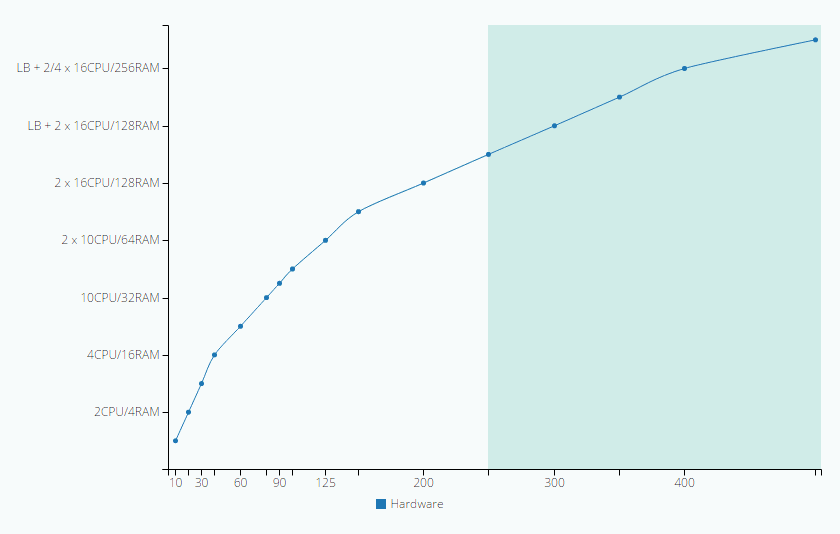
\includegraphics[width=15cm,keepaspectratio]{images/odoo_server_requirments_graph.png}
\caption{Odoo server requirements}
%\source{Source: Michael Aldrich Archive}
\label{pre-production-fig}
\end{figure}

\subsection{Software Requirements}

\begin{description}
	\item[Postgresql v14.0:] Is a powerful, open source object-relational database
	\item[Odoo community v14:] Is a suite of business management software tools
	\item[Docker:] Is a set of platform as a service products that use OS-level virtualization to deliver software in packages called containers
	\item[Docker compose:] Is a tool for defining and running multi-container Docker applications
	\item[Python v3.7] Is a high-level, interpreted, general-purpose programming language.
\end{description}








